% !TEX TS-program = pdflatex
% !TEX encoding = UTF-8 Unicode
% !TEX root = ../main.tex
% !TEX spellcheck = en-US
% ****************************************************************************************
% File: introduction.tex
% Author: Jakob Spindler
% Date: 2024-10-16
% ****************************************************************************************
\chapter{Introduction}
\label{chapter:introduction}

The aim of this report is to investigate the \gls{acr:emc}, more specifically the conducted emissions of a Buck converter in an LTSpice simulation environment \autocite{LTspiceInformationCenter}. The report is largely based on a guide by analog devices \autocite{HowGetBest} and investigates a LT8618 chip \autocite{LT8618DatasheetProduct}.

The following \autoref{fig:no_nothing_schematic} shows the basic setup of the buck converter. The left part of the schematic shows a \gls{acr:lisn} which provides a standardized supply voltage to the converter whilst also enabling the measurement of \gls{acr:dm} - and \gls{acr:cm} conducted emissions.

The \GLS{acr:dm} and \GLS{acr:cm} emissions can be maeasured via the V1 and V2 terminals by using the following expressions:

\begin{equation}
    DM = \frac{V1 - V2}{2}
\end{equation}
\begin{equation}
    CM = \frac{V1 + V2}{2}
\end{equation} 

The right part of the schematic shows the buck converter with its associated components according to its typical application. The ouput capacitor C8 (\qty{4.7}{\micro\farad}) is modelled with a series resistance of \qty{3.82}{\milli\ohm} and a series inductance of \qty{0.7}{\nano\henry} according to the datasheet.
The capacitors C10 (\qty{5}{\pico\farad}) and C11 (\qty{100}{\pico\farad}) are used to model the parasitics of the cooling plate and the case, respectively. Ultimately, the whole setup is loaded with a \qty{200}{\ohm} resistor.

\autoref{fig:no_nothing_emc} shows the conducted emissions of the buck converter. The blue curve represents the \gls{acr:cm} emissions, the green curve the \gls{acr:dm} emissions in \unit{dB\micro\volt}. The red line represents the conducted emissions limt according to the EN 55022/32 standard \autocite{hegartyReviewEMIStandards2018}.
The emissions exceed the limit for frequencies higher than \qty{200}{\kilo\hertz}.

\begin{figure}[h]
    \centering
    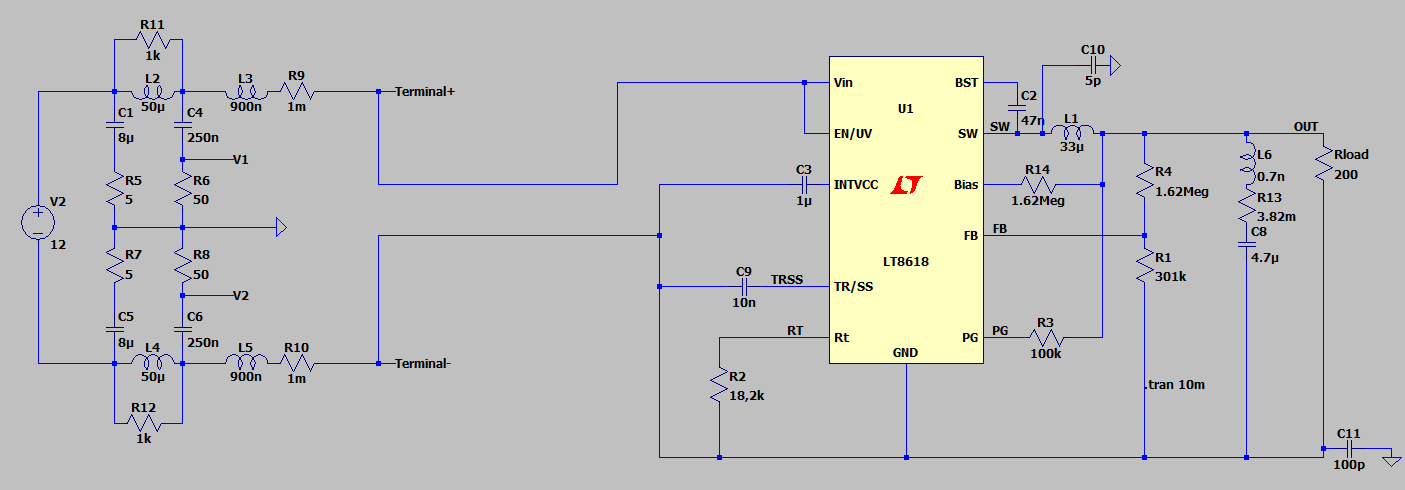
\includegraphics[width=0.8\textwidth]{img/schematic_no_nothing.png}
    \caption{Schematic: \GLS{acr:lisn} and buck converter in their basic setup}
    \label{fig:no_nothing_schematic}
\end{figure}

\begin{figure}[h]
    \centering
    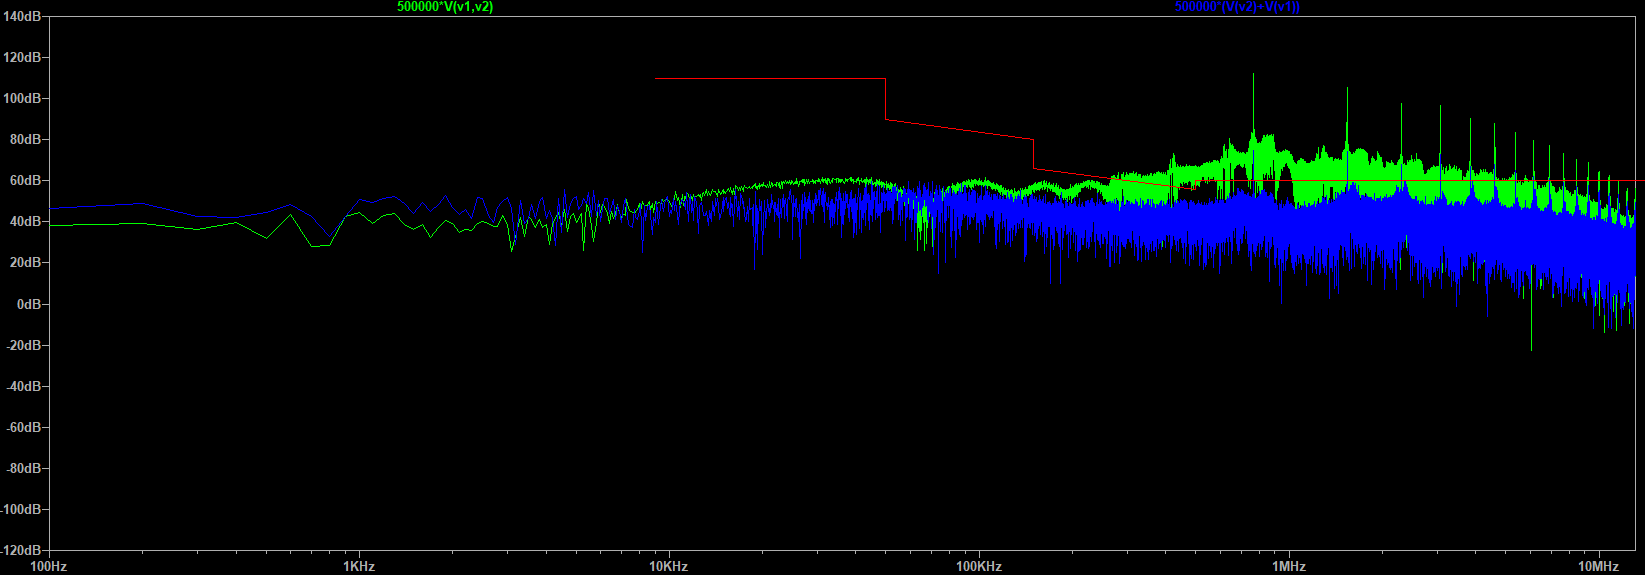
\includegraphics[width=0.8\textwidth]{img/emc_no_nothing.png}
    \caption{conducted emissions of the buck converter - \GLS{acr:dm} in green and \GLS{acr:cm} in blue, red line represents the conducted emissions limit}
    \label{fig:no_nothing_emc}
\end{figure}



% EOF